\section{Analysis}\frame{\sectionpage}

%first slide
\subsection{Basis}
\begin{frame}{Stallman's Argument: Basis}
  \begin{column}{0.5\textwidth}
    \begin{itemize}
      \item A deontological standpoint
      \item Stallman as an ethical essentialist
        \begin{itemize}
          \item proprietary software
          \item restricted data formats
          \item internet services
          \item surveillance
        \end{itemize}
        \begin{itemize}
          \item ``always bring up [free software] as an ethical issue''~\cite[para. 63]{rms2011}
        \end{itemize}
    \end{itemize}
  \end{column} %\hfill
  \begin{column}{0.40\textwidth}\raggedleft{}
    \begin{figure}
      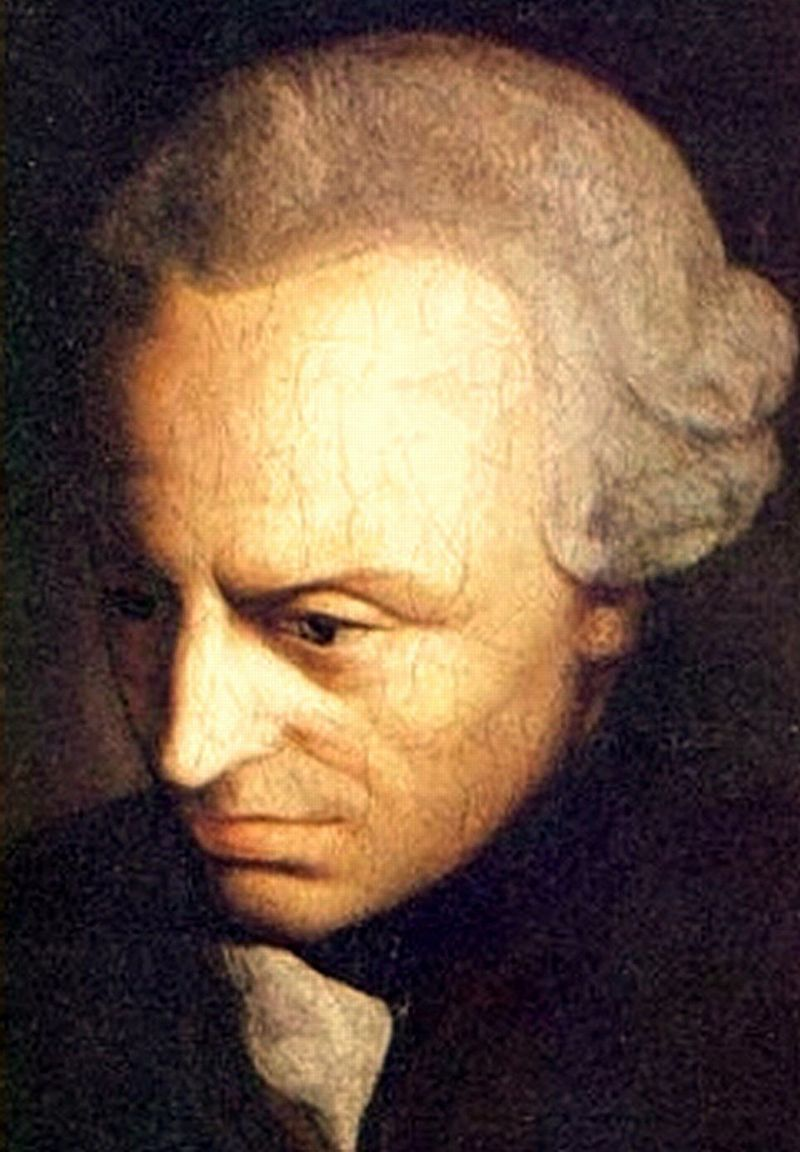
\includegraphics[width = 0.75\textwidth]{images/kant.jpg}
      \caption{\Protect\cite{kant}}
    \end{figure}
  \end{column}
\end{frame}


\subsection{Logos}
\begin{frame}{Stallman’s Argument: Logos}
  \begin{itemize}
    \item Deductive reasoning
      \begin{itemize}
        \item tobacco and proprietary software comparison~\cite[para. 55]{rms2011}
      \end{itemize}
    \item Contradictory premises
      \begin{itemize}
        \item dismissing economics of free digital society (para. 34)
        \item later addressing economics of digital media (para. 109)
      \end{itemize}
  \end{itemize}
\end{frame}

\subsection{Pathos}
\begin{frame}{Stallman’s Argument: Pathos}
  \begin{itemize}
    \item Use of strong characterizations
      \begin{itemize}
        \item ``Computers are Stalin’s dream''~\cite[para. 3]{rms2011}
        \item All DRM should be illegal (para. 30)
      \end{itemize}
    \item Strong appeals to tradition
      \begin{itemize}
        \item values derived from a non-digital society
        \item Amazon Kindle (para. 98)
      \end{itemize}
    \item Calls Amazon Kindle (para. 98)
      \begin{itemize}
        \item an immediate end to digital surveillance
        \item “you can’t wait until there is another dictator” (para. 13)
      \end{itemize}
  \end{itemize}
\end{frame}

